\chapter{Language-augmented multi-agent learning} 

\section{Additional training results on Predator-Prey}\label{app:LAMAC:results}

\begin{figure}[h]
    \centering
    \includesvg[width=\linewidth]{Figures/LAMAC/trainSA15.svg}
    \caption{Training performance in the 15x15 version of Predator-Prey (15 runs each, with median and confidence interval 95\% shown). No variant is able to find a successful strategy in this larger environment when trained from scratch. They all converge towards the suboptimal strategy of avoiding preys to prevent penalties from missed captures. This results in a final return of -1: $T\times p_{step} = 100 \times -0.01$, with $T$ the number of steps in the episode and $p_{step}$ the penalty for each step.}
    \label{fig:trainSA15}
\end{figure}


\clearpage

\section{Implementation details}\label{app:LAMAC:archi}

\subsection{Detailed agent architecture}

\begin{figure}[h]
    \centering
    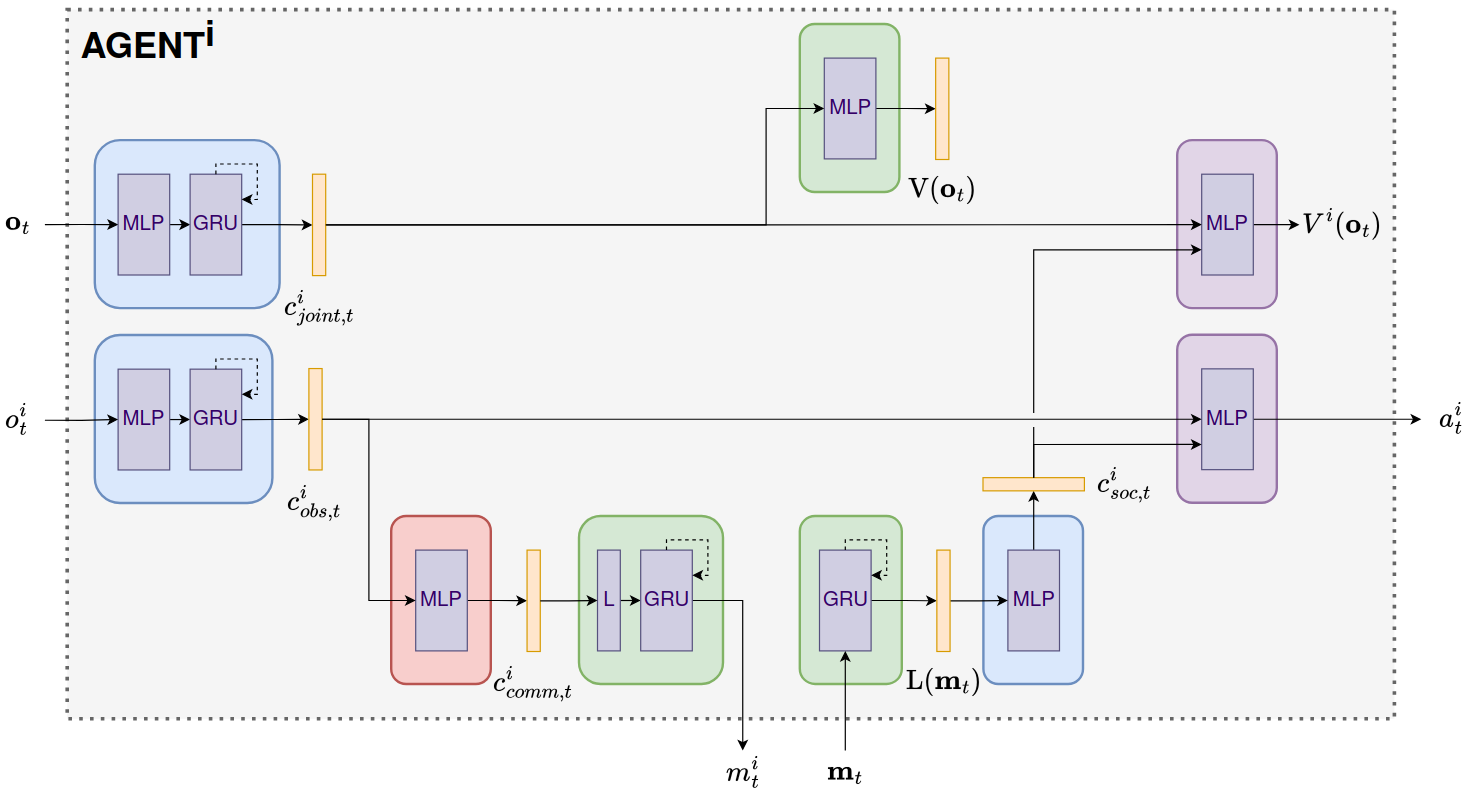
\includegraphics[width=\linewidth]{Figures/LAMAC/archi_detail.png}
    \caption{Detailed architecture of the language-augmented architecture presented in Section~\ref{fig:LAMAC:archi}. Neural networks are shown in purple, with MLP for multi-layer perceptron, GRU for gated recurrent unit, and L for a single neural network layer. All MLPs and GRUs have two hidden layers. }
    \label{fig:App_LAMAC_archi}
\end{figure}

\clearpage
\subsection{Hyperparameters}

\begin{table}[h]
    \centering
    \caption{Hyperparameters used for training the different agent versions.}
    \label{app:App_LAMAC_hyperparam}
    \begin{tabular}{|cccccc}
        \hline
        \multirow{2}{*}{Hyperparameter}  & \multicolumn{5}{|c|}{Algorithm} \\ \cline{2-6} 
                        & \multicolumn{1}{|c}{No Comm}     & \multicolumn{1}{c}{Em-Cont}     & \multicolumn{1}{c}{Em-Disc} & Oracle & \multicolumn{1}{c|}{Lang} \\ \hline 
        \multicolumn{6}{c}{$\varepsilon$-oracle strategy}  \\   \hline
        \multicolumn{1}{|c|}{$\sigma$}   & - & - & - & - & \multicolumn{1}{c|}{$2$}  \\  \hline
        
        \multicolumn{6}{c}{Language training}  \\   \hline
        \multicolumn{1}{|c|}{Lang. batch size}   & - & - & - & \multicolumn{2}{c|}{$1024$}  \\
        \multicolumn{1}{|c|}{Embedding dimension}   & - & - & - & \multicolumn{2}{c|}{$4$}  \\
        \multicolumn{1}{|c|}{Learning rate} & - & - & - & \multicolumn{2}{c|}{$0.007$}  \\   \hline
        
        \multicolumn{6}{c}{Agent architecture}  \\   \hline 
        \multicolumn{1}{|c|}{Context dimension $C$}       & -  & 2     & 16      & 16  & \multicolumn{1}{c|}{$16$}     \\ 
        \multicolumn{1}{|c|}{Hidden dimension $H$}   & \multicolumn{5}{c|}{$64$}  \\  \hline
        
        \multicolumn{6}{c}{PPO training}  \\   \hline
        \multicolumn{1}{|c|}{Nb. of parallel rollouts} & \multicolumn{5}{c|}{$250$}  \\ 
        \multicolumn{1}{|c|}{Learning rate} & \multicolumn{5}{c|}{$0.0005$}  \\ 
        \multicolumn{1}{|c|}{Nb. of PPO epochs} & \multicolumn{5}{c|}{$15$}  \\ 
        \multicolumn{1}{|c|}{Nb. of mini-batches} & \multicolumn{5}{c|}{$1$}  \\
        \multicolumn{1}{|c|}{Nb. of warm-up steps} & \multicolumn{5}{c|}{$50000$}  \\ \hline
    \end{tabular}
\end{table}

In Table~\ref{app:App_LAMAC_hyperparam}, we present the main hyperparameters used in the experiments of Chapter~\ref{ChapterComm}. For training with PPO, many other hyperparameters are used, but we show only the ones that differ from the original implementation. The $\sigma$ parameter used for the $\varepsilon$-oracle strategy (as described in the next section) is fixed to 2 in all experiments. Specific hyperparameters are defined for training the language modules: the sizes of the batches, the dimension of the embedding layers in the decoder and language encoder, and the learning rate applied on these modules. In the agent architecture, the context dimension $C$ used for $c^i_{comm}$ and $c^i_{soc}$, defined in Section~\ref{sec:LAMAC:Archi}, is set to 16 in all language-based agents and the \texttt{Emergent-Discrete} agents, as they use the same architecture as the language-based agents. For the \texttt{Emergent-Continuous} agents, it is set to 2, as $c^i_{comm}$ serves as a continuous message. Larger values were also tried (4, 6, 8, and 16), but they performed worse. For the training of agents with the objective of PPO, we use 250 parallel rollouts: i.e., 250 parallel episodes run between each training phase. Each training phase has 15 consecutive training updates with 1 mini-batch (i.e., all the data collected during rollouts is used in one single batch). Finally, we begin training with a "warm-up" phase of 50000 steps, during which the learning rate is lowered by a factor of $10^{-2}$. 

% \subsection{PPO implementation tricks}




\section{$\varepsilon$-oracle parameter decay}\label{app:LAMAC:param_decay}

In the $\varepsilon$-oracle communication strategy (described in Section~\ref{sec:LAMAC:CommEps}), the parameter $\varepsilon$ is decayed throughout training with a sigmoid-like function defined by:
\begin{equation}
    \varepsilon(t)=\frac{1}{\left[ 1 + e^{-\frac{16}{\sigma}\left( 1 - \frac{t}{T} \right)} \right]^{20}},
\end{equation}
with $t$ the current step of training, $T$ the total number of training steps planned, and $\sigma$ the parameter for controlling the rate of the decay (shown in Figure~\ref{sec:LAMAC:CommEps}), fixed to 2 in our experiments. 
